\SourceLeaf{168}gelingt alle Hindernisse zu übersteigen. Ich würde dann mit der
innigsten Freude alles thun, um Dein Verdienst gelten zu machen und
ins Licht zu stellen, so viel in meinen Kräften steht. Ich komme nun
sogleich zur Sache.

Bei allen \textls{übrigen} Schlüssen finde ich gar nichts wesentliches
einzuwenden: was mich \textls{nicht} 
überzeugt hat, ist bloss das Räsonnement im XIII Artikel. Du denkst
Dir daselbst eine ins Unbestimmte fortgeführte Linie $\Pi\dots kdcfg\dots$,
die aus lauter geraden und gleichen Stücken besteht: $kd$, $dc$, $cf$,
$fg$ etc., und wo die Winkel $kdc$, $dcf$, $cfg$ etc. einander gleich
sind, und willst beweisen, dass $\Pi$ über kurz oder lang nothwendig
über $k\varphi$ hinaus gehen werde. Zu dieser Absicht lässest Du die
gerade Linie $kd\infty = Q$ sich nach der Seite zu, wo $\Pi$ liegt,
um $k$ herumbewegen, so dass sie nach und nach von einer Seite des
Polygons $\Pi$ zur folgenden kommt. Du zeigst vortrefflich, dass $Q$
so, wie es stufenweise durch $d, c, f, g$ etc. geht, jedesmal näher
an $k\varphi$ kommt: gegen alles diess lässt sich
\textls{Nichts} 
einwenden: aber nun fährst Du fort
\begin{center}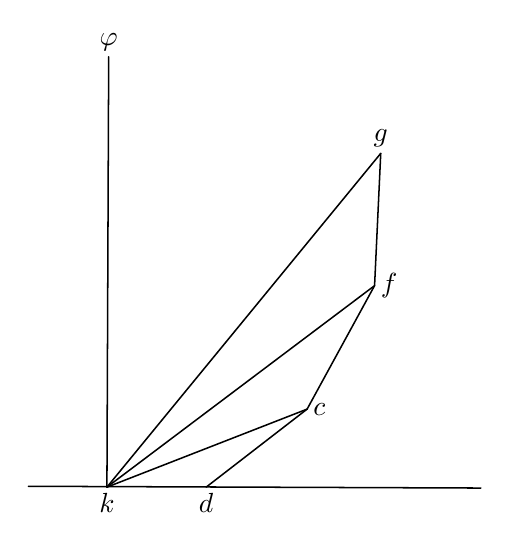
\begin{tikzpicture}[x=1.12cm,y=1.12cm,line width=.55pt,line cap=round,line join=round]
\coordinate (k) at (0,0);
\coordinate (d) at (1.125,0);
\coordinate (c) at (2.27,.885);
\coordinate (f) at (3.035,2.285);
\coordinate (g) at (3.105,3.785);
\coordinate (phi) at (.02,4.88);
\draw (-.89,.01)--(4.24,-.01);
\draw (k)--(phi);
\draw (k)--(c);
\draw (k)--(f);
\draw (k)--(g);
\draw (d)--(c)--(f)--(g);
\node[above,inner sep=2pt] at (phi) {$\varphi$};
\node[above,inner sep=2pt] at (g) {$g$};
\node[right,inner sep=2pt] at (f) {$f$};
\node[right,inner sep=2pt] at (c) {$c$};
\node[below,inner sep=2pt] at (d) {$d$};
\node[below,inner sep=2pt] at (k) {$k$};
\end{tikzpicture}
\end{center}
\begin{quote}
»Quapropter $Q$ moveri potest modo praescripto usque dum in
$k\varphi$, $\varphi\infty$ pervenerit« etc.
\end{quote}
und diese Schlussfolge ist es, die mir nicht einleuchtet. Aus Deinem
Räsonnement folgt, meiner Einsicht nach, noch gar nicht, dass der
Winkel, um den $Q$, beim Durchlaufen einer Seite von $\Pi$ (nach oben
herum), der $k\varphi$ näher kommt, nicht etwa immer unbedeutender
werde, so dass das Aggregat aller successiven Annäherungen, so oft
sie auch wiederholt werden, dennoch immer noch nicht gross [genug]
werden könnte, um $Q$ in $k\varphi$ zu bringen. Könntest Du \textls{beweisen},
dass $dkc = ckf = fkg$ etc., so wäre die Sache gleich aufs Reine.
Aber dieser Satz ist zwar wahr, allein schwerlich ohne die Theorie
der Parallelen schon vorauszusetzen, strenge zu beweisen. Man könnte
also immer noch besorgen, dass die Winkel $dkc$, $ckf$, $fkg$ etc.
successive abnehmen. Geschähe diess (bloss \textls{exempli gratia}) in einer
geometrischen Progression, so dass $ckf = \psi \times dkc$,
$fkg = \psi \times dkc$ etc. (so dass $\psi$ kleiner als 1), so würde
